\documentclass{article}

\usepackage{tikz}

\begin{document}

This is a document with a picture or two.

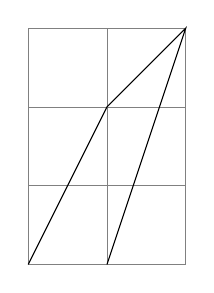
\begin{tikzpicture}
  \draw[help lines] (0,0) grid (2,3);
  \draw (0,0) -- (1,2) -- (2,3) -- (1,0);
\end{tikzpicture}

Let me try labelling:

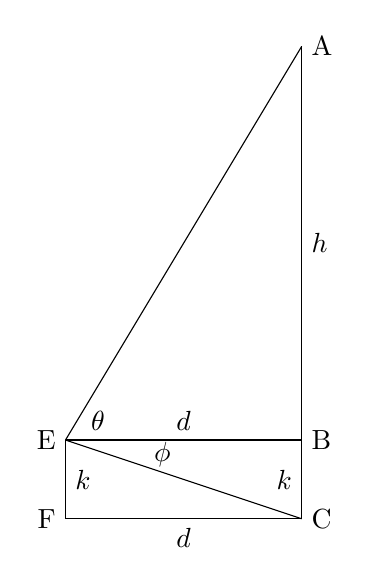
\begin{tikzpicture}
  \draw (0,0) -- (0,1);
  \draw (3,0) -- (3,6);
  \draw (0,0) -- (3,0);
  \draw (0,1) -- (3,0);
  \draw (0,1) -- (3,6);
  \draw (0,1) -- (3,1);
  % vertices
  \node[left] at (0,1) {E};
  \node[left] at (0,0) {F};
  \node[right] at (3,6) {A};
  \node[right] at (3,1) {B};
  \node[right] at (3,0) {C};
  % line lengths
  \node[below] at (1.5,0) {$d$};
  \node[above] at (1.5,1) {$d$};
  \node[right] at (0,0.5) {$k$};
  \node[left] at (3,0.5) {$k$};
  \node[right] at (3,3.5) {$h$};
  % angles
  \node[above right] at (0.2,1) {$\theta$};
  \node[below right] at (1,1.1) {$\phi$};
\end{tikzpicture}

and the same but bigger:

\begin{tikzpicture}[scale=2]
  \draw (0,0) -- (0,1);
  \draw (3,0) -- (3,6);
  \draw (0,0) -- (3,0);
  \draw (0,1) -- (3,0);
  \draw (0,1) -- (3,6);
  \draw (0,1) -- (3,1);
  % vertices
  \node[left] at (0,1) {E};
  \node[left] at (0,0) {F};
  \node[right] at (3,6) {A};
  \node[right] at (3,1) {B};
  \node[right] at (3,0) {C};
  % line lengths
  \node[below] at (1.5,0) {$d$};
  \node[above] at (1.5,1) {$d$};
  \node[right] at (0,0.5) {$k$};
  \node[left] at (3,0.5) {$k$};
  \node[right] at (3,3.5) {$h$};
  % angles
  \node[above right] at (0.1,1) {$\theta$};
  \node[below right] at (0.5,1.05) {$\phi$};
\end{tikzpicture}


\end{document}
